\begin{figure}[t!]
  \begin{center}
    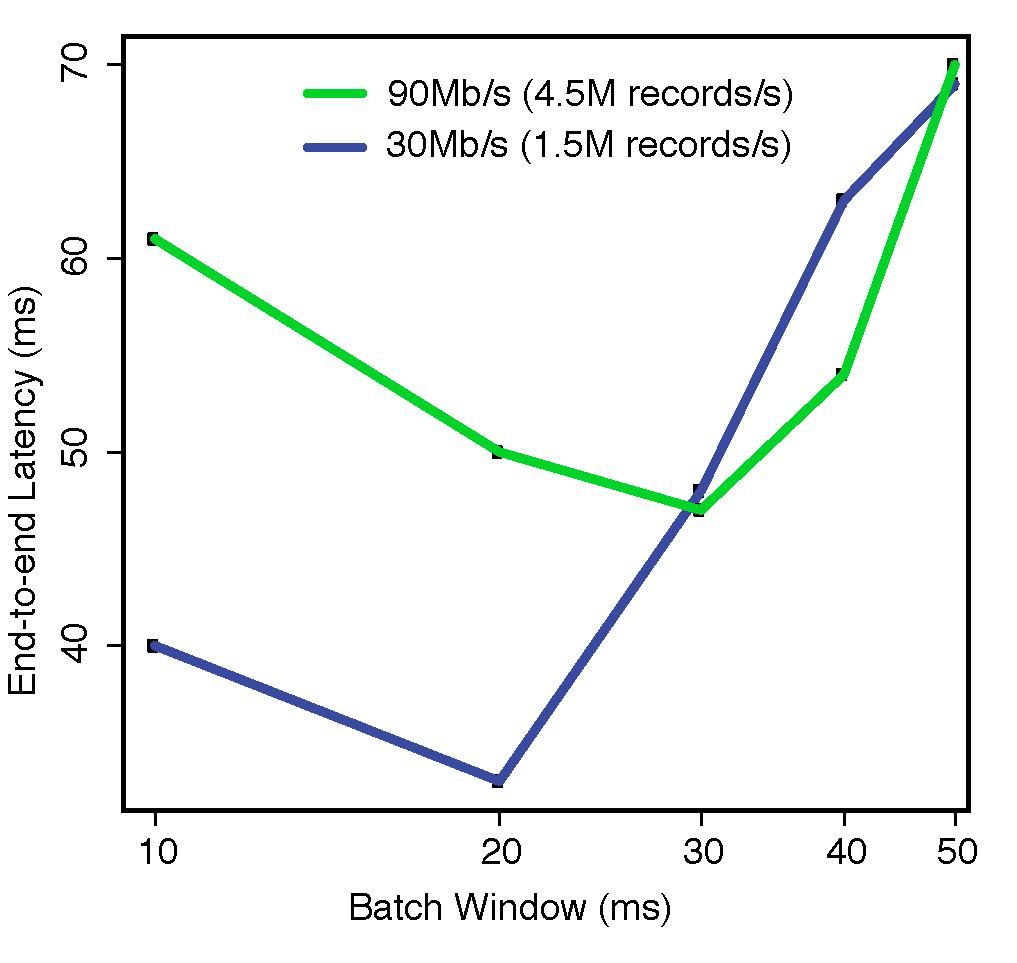
\includegraphics[scale=0.35]{images_graphs/batchsize_vs_latency/batchsize_vs_latency_illustrator.pdf}
  \end{center}
  \caption{Average end-to-end latency for different batch window sizes and different throughputs}
  \label{fig:Batchsize_vs_latency}
\end{figure}



To better understand the performance and limitations of Spark Streaming we conducted a benchmark study of the system.

To this end we have instrumented Spark Streaming.
Our instrumentation code allows us to track a subset of the stream data as it flows through the system.
We record at which moments of time some of the records pass through some of the components.

To exercise Spark Streaming we have used a synthetic workload.
%To this end we used a synthetic workload to exercise Spark Streaming and measure how the system behaves under different scenarios.
This workload consists of an application that listens for a stream of text records.
Each record has size between 15-25 bytes and holds a unique ID and a timestamp of time when the data was generated.
For each micro-batch, the application computes and records the end-to-end latency of the first 10 records in the micro-batch.

The computation performed by this workload is very lightweight.
We believe that this is in line with the type of computations used with Spark Streaming.
First, typical streaming tasks consist of filtering and/or simple aggregations.
These are operations that scale linearly with the amount of data in each batch.
Secondly, there is extensive work on optimizing the performance of query processing, both in batch and streaming contexts.
Finally, many steps of the computations performed in Spark and Spark Streaming are embarrassingly parallel. 
This means that developers can make use of more hardware to get better performance. 

%This is because first, the computation time is almost always orthogonal to the architecture used.
%Secondly, there is other work aimed at improving computation times in streaming or MapReduce systems.
%    There is parallel work on improving the performance of streaming computations that can be used to improve the execution times of tasks.

To run this benchmark, we have deployed a Receiver and a record generator in two different machines in the same cluster.

The record generator generates as many records as necessary to achieve a user-specified throughput.
Each record contains a timestamp that corresponds to the moment of creation of the record as well as a unique ID.
The Receiver uses the Spark Streaming API to consume this data. 
A task is generated periodically, according to a user-defined frequency, and scheduled to a node where the data is processed.

\begin{figure}[t!]
  \begin{center}
    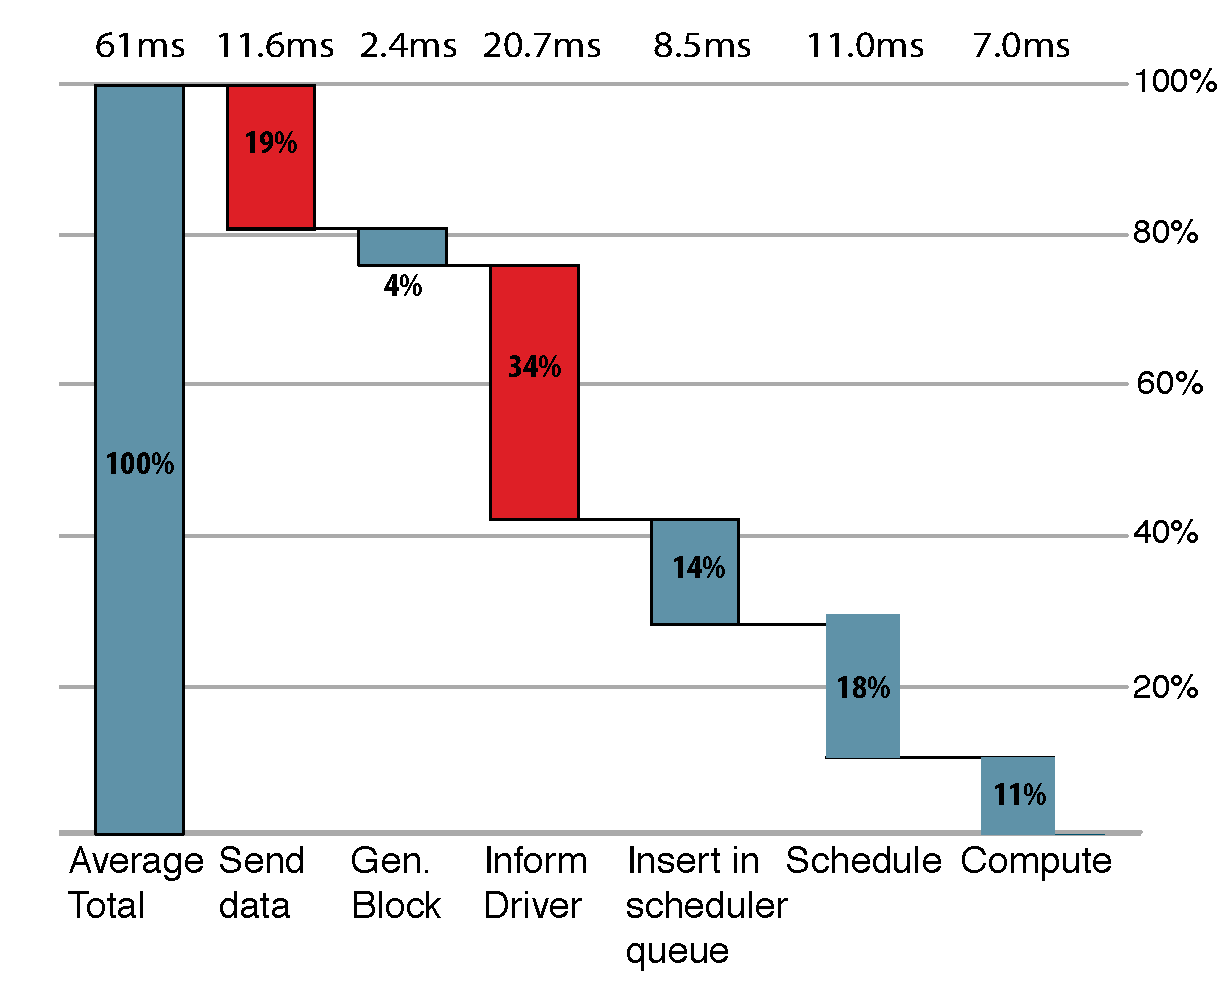
\includegraphics[scale=0.40]{images_graphs/waterfall/Rplots_illustrator.pdf}
  \end{center}
  \caption{Execution time breakdown for a batch window of 10ms at 90MB/s}
  \label{fig:SparkStreaming_time_breakdown}
\end{figure}

\begin{figure}[t!]
  \begin{center}
    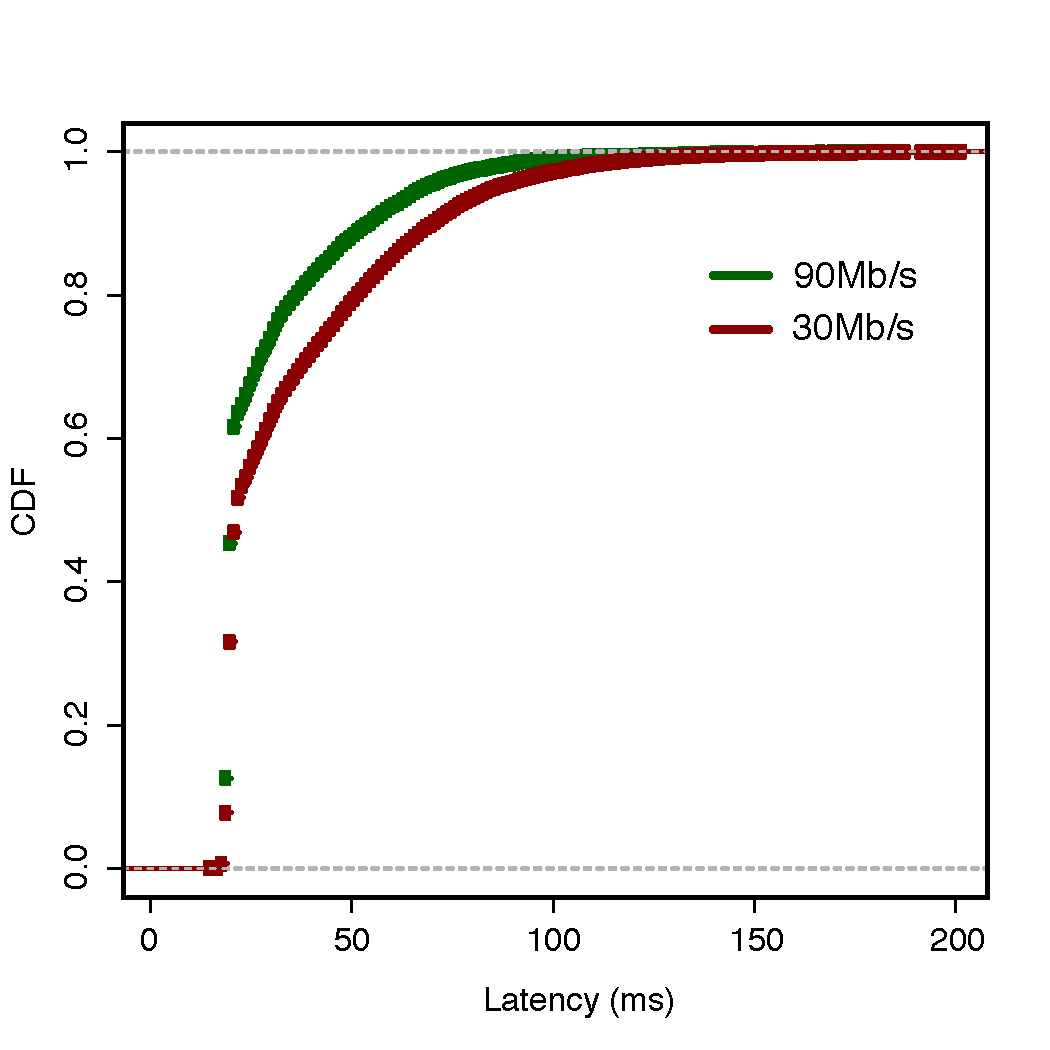
\includegraphics[scale=0.40]{images_graphs/cdf_latencies/cdf_e2e_times.pdf}
  \end{center}
  \caption{CDF of latencies for a batch window of 10ms at 90MB/s and 30MB/s}
  \label{fig:CDF_latencies}
\end{figure}

We have instrumented the code of Spark Streaming to record the time at which the record transitions a phase (e.g., a task to process a record is scheduled).
%#understand how much time each record stays on each phase of the streaming process.
This allows us to gather 1) the time each record spends on each phase of the streaming process, and 2) the time between the generation of each record and the moment of computation -- end-to-end latency.

%When processing records, the time between the generation of each record and the moment of computation is captured. 
%We refer to this value throughout the paper as the end-to-end latency. 

The results of the first experiment we conducted are captured in Figure~\ref{fig:Batchsize_vs_latency}.
In this graph we show the average end-to-end latency obtained when running Spark Streaming with five different batch window configuration values and two different throughput levels.
Changing the batch window configuration allows us to tune the responsiveness of the system;
a lower value means that each records spends less time in memory waiting for a task to be spawned in order to process that same record. 
Varying the number of records generated by the stream source (throughput), allows us to understand how 
Spark behaves when it has to do more/less work per unit of time and how that affects latency.

As expected, as we instruct Spark Streaming to spawn tasks more frequently -- smaller batch window -- the average end-to-end latency time decreases.
However, at some point decreasing the batch window has a negative effect on the resulting latency.
Moreover, as we increase the throughput the end-to-end latency increases.
We have found that the Spark Streaming's Receiver can be a source of slowdown.
For instance, we found that it is not able to receive more than roughly 30 MB/s (1.5M records).
This has to do with the fact that this component receives and stores data in a streaming fashion.
For batch windows less than 10ms we found the system to be unstable, and the latency increases indefinitely.

Next, to understand where time is spent we decomposed the execution time of Spark Streaming in different phases.
We provide this result in figure~\ref{fig:SparkStreaming_time_breakdown}. 
-- this corresponds to the top left point of figure~\ref{fig:Batchsize_vs_latency} (batch window is 10ms and throughput is 90MB/s).
This graph provides several insights. First, roughly 20\% of the time is spent waiting for data to be transmitted from the source of data to the Receiver.
This time has to do with the architecture of the Receiver, as it was already explained.
Second, a third of the time is spent between generating a block of data and informing the driver about blocks received.
This time stems from the fact that the Driver creates only one thread for handling the receival of metadata about blocks.
In workloads with several receivers and a high number of blocks generated per unit of time, this single thread is not able to respond 
